\chapter{Introduction}\label{ch:introduction}

Robots have been massively introduced in the field of manufacturing around the eighties, but ever since they have been mainly used in very fixed and structured environments and with no or rare interaction of robots with human workers. Nowadays new kind of robotic manipulators, including dual arm setups and mobile manipulators, are being rolled out from bigger producers such as KUKA, ABB, Universal Robots, Rethink Robotics and more, featuring lightweight and compliant structures that can be exploited to tackle the upcoming needs of the new Industry 4.0 paradigm where cyber-physical systems communicate and cooperate with each other and humans in real time. These trends have been especially identified, in the European Multi-Annual Roadmap for robotics, as innovations with high potential impact on market domains \cite{mar2020} and covered in a series EU H2020 calls, such as the recent ICT (Information and Communication Technology) one on \textit{Advanced robot capabilities} research \cite{h2020AdvRobCall}.
Towards that end, the control of the robot must be able to guarantee a high level of flexibility in order to accomplish a variety of tasks that go beyond the usual, standardized, robotic cell ones, which use to take place within a very structured environment. The basic idea is that the robot should autonomously take care of all the control objectives related to the safety of the system, interaction with the environment, as well as those that are a prerequisite to accomplish the required task. Achieving these objectives would indeed grant the robot a higher level of flexibility, simplifying the higher levels that deal with planning and task sequencing.

\begin{figure}
	\centering
	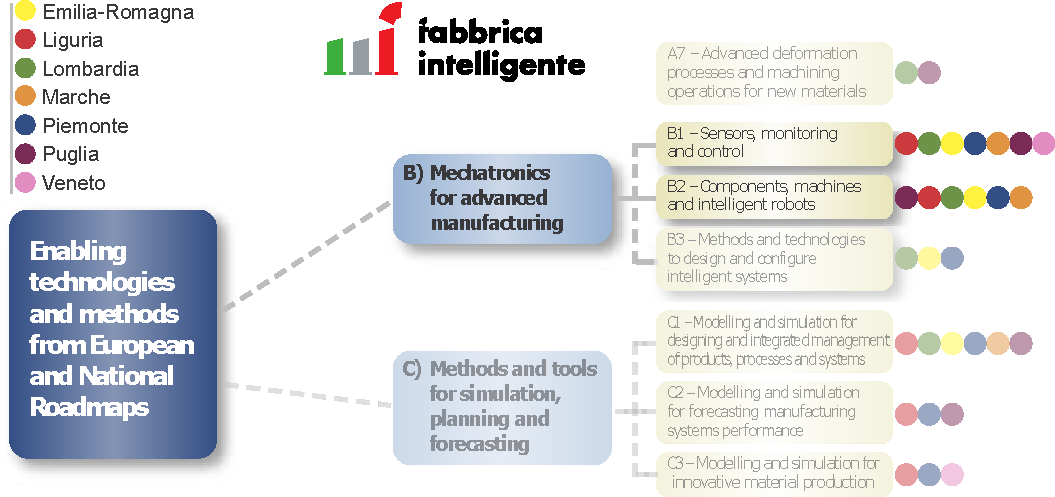
\includegraphics[width=0.8\textwidth]{images/intro/framing_CFI}
	\caption{A focused extract from the Italian ``\textit{Research and Innovation Roadmap}'' \cite{CFIRoadmap} for smart manufacturing, highlighting the scope in which this PhD work is framed.}
	\label{fig:cfi}
\end{figure}

This PhD work is in fact framed within the Italian technology cluster \textit{Fabbrica Intelligente} (i.e. Smart Manufacturing). In particular, as seen in figure \ref{fig:cfi}, in the Italian ``\textit{Research and Innovation Roadmap}'' \cite{CFIRoadmap}, a series of the key enabling technologies have been identified in the are of ``Mechatronics for advanced manufacturing'', where the Liguria region in which our university resides, is involved in the development of \textit{Sensors, monitoring and control} and  \textit{Components, machines and intelligent robots}.



\section{State of the art and innovation}
Redundant robotic systems are becoming increasingly more...
